\documentclass[11pt,a4paper]{amsart}
\usepackage{amssymb, amstext, amscd, amsmath}
\usepackage{tikz}
\tikzset{nodeblack/.style={circle,draw=black,fill=black!30,inner sep=1.2pt}}
\tikzset{every loop/.style={}}

\begin{document}

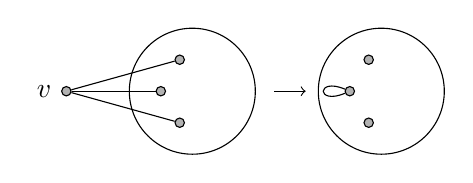
\begin{tikzpicture}[scale=0.8]
% Left-side nodes (x, y, z) and connecting node v
\node[nodeblack] at (-0.2,2.5) (x) {};
\node[nodeblack] at (-0.5,2) (y) {};
\node[nodeblack] at (-0.2,1.5) (z) {};
\node[nodeblack, label=left:$v$] at (-2,2) (v) {};

% Edges from v to x, y, z (defined after all involved nodes exist)
\draw (v) -- (x);
\draw (v) -- (y);
\draw (v) -- (z);

% Left circle centered at (0,2)
\draw (0,2) circle (1cm);

% Arrow between the two circles
\draw[->] (1.3,2) -- (1.8,2);

% Right circle centered at (3,2)
\draw (3,2) circle (1cm);

% Right-side nodes (x1, y1, z1)
\node[nodeblack] at (2.8,2.5) (x1) {};
\node[nodeblack] at (2.5,2) (y1) {};
\node[nodeblack] at (2.8,1.5) (z1) {};

% Loop on y1 (must come after y1 is defined)
\path (y1) edge[in=157, out=203, loop] ();

\end{tikzpicture}

\end{document}